\chapter{Ανάλογα ποσά - Αντιστρόφως ανάλογα ποσά}
\begin{exercise}
Να σχεδιάσεις ένα ορθοκανονικό σύστημα ημιαξόνων, με μονάδα το 1 cm και να
τοποθετήσεις τα σημεία Α(2,3), Β(3,2), Γ(4,5), Δ(5,5), Ε(1,4), Z(7,3), Η(7,2), Θ(6,2),
Ι(6,0), Κ(0,5). Τι παρατηρείς για τα σημεία Ι και Κ; Πού βρίσκονται αυτά; Μπορείς να
γενικεύσεις τις παρατηρήσεις σου για τα σημεία που έχουν τετμημένη ή τεταγμένη το
μηδέν;
\end{exercise}
\begin{lstlisting}
import matplotlib.pyplot as plt

plt.clf()
points = [(2,3), (3,2), (4,5), (5,5), (1,4), (7,3), (7,2), (6,2), (6,0), (0,5)]
pointName = ['Α','Β','Γ','Δ','Δ','Ε','Ζ','Η','Θ','Ι','Κ']
x = [p[0] for p in points]
y = [p[1] for p in points]
color=['m','g','r','b']
plt.grid()
plt.scatter(x,y, s=100 ,marker='o', c=color)
for (i,p) in enumerate(points):
    plt.annotate(pointName[i],(p[0],p[1]))

plt.show()
\end{lstlisting}
\begin{figure}
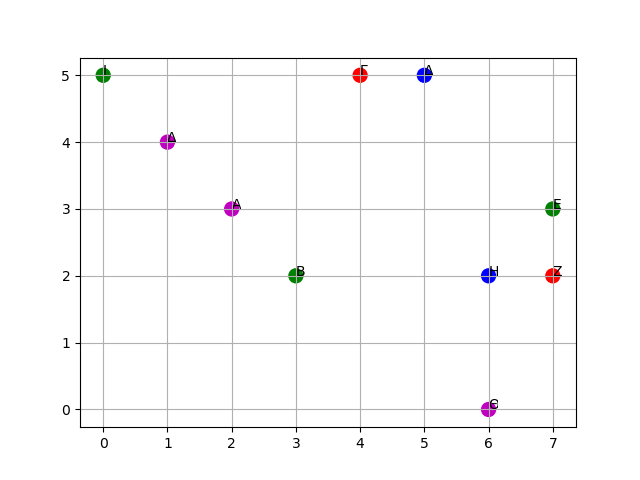
\includegraphics{graph1.png}
\end{figure}
\begin{exercise}
\sel[2]{89}
Σε ορθοκανονικό σύστημα ημιαξόνων να τοποθετήσεις τα σημεία Α(2,1), Β(1,2), Γ(2,3)
και Δ(3,2). Τι σχήμα είναι το ΑΒΓΔ; Αν τα ευθύγραμμα τμήματα ΑΓ και ΒΔ τέμνονται
στο σημείο Κ, ποιες είναι οι συντεταγμένες του Κ;
\end{exercise}
\begin{lstlisting}
import matplotlib.pyplot as plt

plt.clf()
points = [(2,1), (1,2), (2,3), (3,2)]
pointName = ['Α','Β','Γ','Δ']
x = [p[0] for p in points]
y = [p[1] for p in points]
color=['m','g','r','b']
plt.grid()
plt.scatter(x,y, s=100 ,marker='o', c=color)
for (i,p) in enumerate(points):
    plt.annotate(pointName[i],(p[0],p[1]))

x = [points[0][0],points[2][0]]
y = [points[0][1],points[2][1]]
plt.plot(x,y)
x = [points[1][0],points[3][0]]
y = [points[3][1],points[3][1]]
plt.plot(x,y)

plt.show()
\end{lstlisting}
\begin{figure}
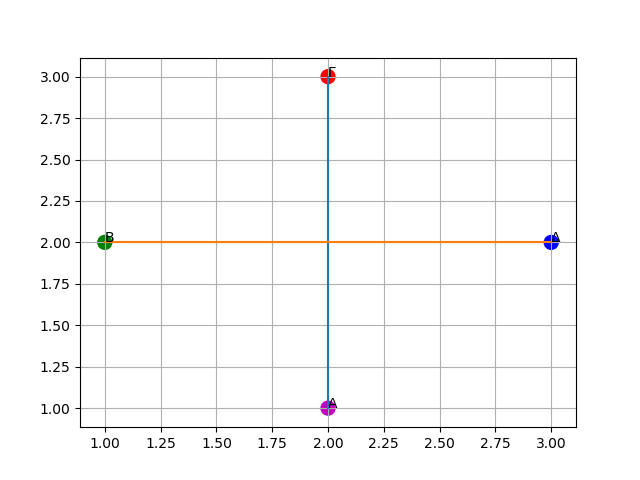
\includegraphics{graph2.png}
\end{figure}

\begin{exercise}
\sel[3]{89}
Γράψε πέντε διατεταγμένα ζεύγη σημείων, των οποίων η τετμημένη τους είναι ίση με
την τεταγμένη τους. Μπορείς να τα
τοποθετήσεις, σε ένα ορθοκανονικό
σύστημα ημιαξόνων; Τι παρατηρείς;
\end{exercise}
\begin{lstlisting}
import matplotlib.pyplot as plt

plt.clf()
points = [(1,1), (2,2), (5,5), (10,10), (15,15)]
pointName = ['Α','Β','Γ','Δ','Ε']
x = [p[0] for p in points]
y = [p[1] for p in points]
color=['m','g','r','b']
plt.grid()
plt.scatter(x,y, s=100 ,marker='o', c=color)
for (i,p) in enumerate(points):
    plt.annotate(pointName[i],(p[0],p[1]))

plt.show()
\end{lstlisting}
\begin{figure}
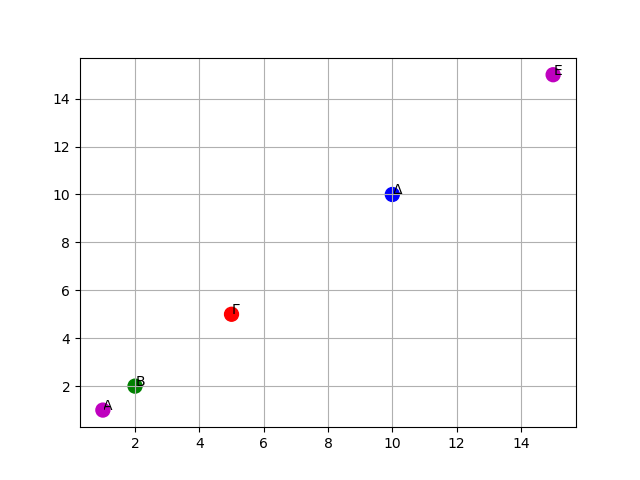
\includegraphics{graph3.png}
\end{figure}

\begin{exercise}
\sel{90}
Συμπλήρωσε τον παρακάτω πίνακα:
\begin{table}
\begin{tabular}{|l|c|c|c|}
Πλευρά τετραγώνου& 1,5 cm& 4 cm& 4,5 cm\\\hline
Περίμετρος τετραγώνου&&&\\\hline
\end{tabular}
\end{table}
\begin{itemize}
\item Εξήγησε πώς προκύπτουν οι αριθμοί της δεύτερης σειράς.
\item Βρες για κάθε τετράγωνο το κλάσμα πλευρά προς περίμετρο.
\item Ποιο είναι το συμπέρασμα που βγάζεις;
\end{itemize}
\end{exercise}
\begin{lstlisting}
>>> 4*1.5
6.0
>>> 4*4
16
>>> 4*4.5
18.0
\end{lstlisting}
\begin{tabular}{|l|c|c|c|}
Πλευρά τετραγώνου& 1,5 cm& 4 cm& 4,5 cm\\\hline
Περίμετρος τετραγώνου&6&16&18\\\hline
\end{tabular}
Θυμηθείτε το ποσοστό σε κλάσμα:
\begin{lstlisting}
def posostoseklasma(fx):
    fx = float(fx)
    denom = 100
    while int(fx) != fx:
         fx *= 10
         denom *= 10
    fx = int(fx)
    return(Fraction(fx,denom))
\end{lstlisting}
Το fx είναι είναι ο αριθμητής ενός κλάσματος με παρονομαστή 100. Εδώ δεν θα υπάρχει ο παρονομαστής 100 οπότε έχουμε denom = 1.
\begin{lstlisting}
def dekadikosseklasma(fx):
    fx = float(fx)
    denom = 1
    while int(fx) != fx:
         fx *= 10
         denom *= 10
    fx = int(fx)
    return(Fraction(fx,denom))

dekadikosseklasma(1.5/6)
dekadikosseklasma(4/16)
dekadikosseklasma(4.5/18)
\end{lstlisting}
και το αποτέλεσμα είναι:
\begin{lstlisting}
>>> dekadikosseklasma(1.5/6)
Fraction(1, 4)
>>> dekadikosseklasma(4/16)
Fraction(1, 4)
>>> dekadikosseklasma(4.5/18)
Fraction(1, 4)
\end{lstlisting}
Άρα παντού το κλάσμα είναι $\frac{1}{4}$.
\begin{exercise}
\sel{90}
Χρησιμοποιούμε τη φωτογραφική μηχανή
για να απεικονίσουμε εικόνες αντικειμένων. Οι εικόνες αυτές δείχνουν τα
πραγματικά αντικείμενα σε σμίκρυνση.
Στη φωτογραφία το ύψος ενός παιδιού
είναι 2 cm ενώ γνωρίζουμε ότι το πραγματικό του ύψος είναι 1,65 m = 165 cm. Πόση θα είναι τότε η σμίκρυνσή του
στη φωτογραφία;
\end{exercise}
\begin{lstlisting}
>>> 2/165
0.012121212121212121
\end{lstlisting}

\begin{exercise}
\sel{91}
Μετρούμε μια απόσταση, σε χάρτη, με κλίμακα 1:10.000.000 και τη βρίσκουμε
ίση με 2,4 cm. Ποια είναι η πραγματική απόσταση των δύο σημείων;
\end{exercise}
\begin{lstlisting}
>>> x = 2.4*10000000
>>> x
24000000
>>> x = x/100
>>> x
240000
>>> x = x/1000
>>> x
240
\end{lstlisting}
240Km
\begin{exercise}
\sel[3]{92}
Σε μια φωτογραφία το ύψος ενός ανθρώπου είναι 4 cm, ενώ το
πραγματικό το ύψος είναι 1,76 m. Πόσο έχει σμικρυνθεί η εικόνα του
ανθρώπου στη φωτογραφία;
\end{exercise}
\begin{lstlisting}
def pososto(x):
    print(str(round(x*100,2))+'%')
\end{lstlisting}
Αν θυμηθούμε τη συνάρτηση pososto τότε
\begin{lstlisting}
>>> pososto(4/176)
2.27%
\end{lstlisting}
\begin{exercise}
\sel[4]{92}Ένας προβολέας διαφανειών προβάλλει το κείμενο μιας διαφάνειας στον απέναντι
τοίχο. Αν ένα ``A'' έχει ύψος 7 mm στη διαφάνεια και 4,2 cm στον τοίχο, ποια είναι η
μεγέθυνση που δίνει ο προβολέας
\end{exercise}
\begin{lstlisting}
>>> pososto(4.2/0.7)
600%
\end{lstlisting}
\begin{exercise}
\sel[5]{92}
Η σύνθεση μιας μπλούζας είναι 80\% βαμβάκι και το υπόλοιπο πολυεστέρας. Aν η μπλούζα
ζυγίζει 820 gr, πόσα γραμμάρια ζυγίζουν τα νήματα του πολυεστέρα που περιέχει;
\end{exercise}
\begin{lstlisting}
>>> 820*20/100
164.0
\end{lstlisting}
\begin{exercise}
\sel[6]{92}
Να συμπληρωθεί ο πίνακας
\begin{table}
\begin{tabular}{|c|c|c|c|c|c|}
\hline
Κλίμακα&1:5&3:8&1:30&&1:100\\\hline
Μήκος σε σχέδιο&4cm &&12cm&2cm&3,5cm\\\hline
Πραγματικό ύψος&&24m&&10m&\\\hline
\end{tabular}
\end{table}
\end{exercise}
\begin{lstlisting}
>>> from fractions import Fraction
>>> 5*4
20
>>> 3/8*24
9.0
>>> 12*30
360
>>> Fraction(2,1000)
Fraction(1, 500)
>>> 3.5*100
350
\end{lstlisting}
Άρα ο πίνακας γίνεται:
\begin{table}
\begin{tabular}{|c|c|c|c|c|c|}
\hline
Κλίμακα&1:5&3:8&1:30&1:500&1:100\\\hline
Μήκος σε σχέδιο&4cm &9cm&12cm&2cm&3,5cm\\\hline
Πραγματικό ύψος&20cm&24m&360cm&10m&350cm\\\hline
\end{tabular}
\end{table}
\begin{exercise}
\sel[7]{92}
Οι διαστάσεις ενός ορθογωνίου παραλληλογράμμου είναι $x+2$ και $x$.

(α) Να γράψεις τη σχέση που συνδέει την περίμετρο Π του ορθογωνίου με το x.

(β) Να συμπληρώσεις τον πίνακα:
\begin{table}
\begin{tabular}{|c|c|c|c|c|}
x&&2&&4\\\hline
Π&8&&16&\\\hline
\end{tabular}
\end{table}
\end{exercise}
α)
\begin{lstlisting}
>>> from sympy import *
>>> x = symbols('x')
>>> p = x+x+2+x+x+2
>>> p
4*x + 4
\end{lstlisting}
β)
\begin{lstlisting}
>>> solve(p-8)
[1]
>>> p.subs(x,2)
12
>>> solve(p-16)
[3]
>>> p.subs(x,4)
20
\end{lstlisting}
και ο πίνακας γίνεται:
\begin{table}
\begin{tabular}{|c|c|c|c|c|}
\hline
x&1 &2  &3  &4\\\hline
Π&8&12&16&20\\\hline
\end{tabular}
\end{table}
\begin{exercise}
\sel[8]{92}
Aν οι διαστάσεις ενός δωματίου, σε ένα σχέδιο με κλίμακα 1:250, είναι 3x5, οι
πραγματικές διαστάσεις του δωματίου θα είναι .....x..... .
\end{exercise}
\begin{lstlisting}
>>> 3*250
750
>>> 5*250
1250
\end{lstlisting}
Οπότε το δωμάτιο είναι 7,5m x 12,5m αν οι διαστάσεις ήταν σε cm.
\begin{exercise}
\sel[9]{92}
Αν ανακατέψουμε 2 κιλά κόκκινο χρώμα και 3 κιλά κίτρινο χρώμα,
φτιάχνουμε μια συγκεκριμένη απόχρωση του πορτοκαλί. Αν
ανακατέψεις 5 κιλά κόκκινο χρώμα και 6 κιλά κίτρινο, θα πάρεις
την ίδια απόχρωση; Δικαιολόγησε την απάντησή σου.
\end{exercise}
\begin{lstlisting}
>>> 3/2 == 6/5
False
\end{lstlisting}
Όχι δεν είναι η ίδια απόχρωση.
\begin{exercise}
\sel[2]{93} Όταν ο Κώστας έκλεισε τα δώδεκα χρόνια είχε το ένα τρίτο της
ηλικίας της μητέρας του. Όταν θα γίνει είκοσι χρόνων, ο λόγος των
δύο ηλικιών τους θα παραμείνει ο ίδιος;
\end{exercise}
\begin{lstlisting}
>>> ilikiaMiteras = 3*12
>>> ilikiaMiteras
36
>>> xronia = 20-12
>>> xronia
8
>>> neailikiaMiteras = ilikiaMiteras + xronia
>>> neailikiaMiteras = 44
>>> 44/20 == 36/12
False
\end{lstlisting}
Άρα όχι.
\begin{exercise}
Να συμπληρωθεί ο πίνακας, αν γνωρίζουμε ότι τα ποσά x και 􀁜 είναι ανάλογα, με
συντελεστή αναλογίας $\alpha = \frac{2}{3}$.
\begin{table}
\begin{tabular}{|c|c|c|c|c|c|c}
\hline
x &0 &1 &0,3& &\\\hline
y &    &  &       & $\frac{5}{3}$ & 3\\\hline
\end{tabular}
\end{table}
\end{exercise}
$$
y = \frac{2}{3}x
$$
\begin{lstlisting}
>>> from sympy import *
>>> (x,y) = symbols('x y')
>>> e = 2/3*x
>>> e.subs(x,0)
0
>>> e.subs(x,1)
0.666666666666667
>>> e.subs(x,0.3)
0.200000000000000
>>> solve(e-5/3)
[2.50000000000000]
>>> solve(e-3)
[4.50000000000000]
\end{lstlisting}
Και ο πίνακας γίνεται:
\begin{table}
\begin{tabular}{|c|c|c|c|c|c|c}
\hline
x &0 &1 &0,3& 2,5&4,5\\\hline
y & 0   & 0,6666 & 0,2      & $\frac{5}{3}$ & 3\\\hline
\end{tabular}
\end{table}
\begin{exercise}
\sel[2]{92}
Σε ένα διάλυμα ζάχαρης η περιεκτικότητα σε ζάχαρη είναι 23\%. Πόσα γραμμάρια
ζάχαρης υπάρχουν σε 300 gr διαλύματος;
\end{exercise}
\begin{lstlisting}
>>> 300*23/100
69.0
\end{lstlisting}
\begin{exercise}
\sel[3]{97}
Ένα πλοίο έχει σταθερή ταχύτητα και καλύπτει απόσταση 80 Km σε 2 ώρες. Σε πόσο
χρόνο θα καλύψει απόσταση 2.000 Km;
\end{exercise}
$$\frac{2}{80}=\frac{x}{2000}$$
\begin{lstlisting}
>>> from sympy import *
>>> x = symbols('x')
>>> solve(2/80-x/2000)
[50.0000000000000]
\end{lstlisting}
Η απάντηση είναι 50 ώρες.
\begin{exercise}
Εξέτασε αν τα ποσά που δίνονται στους παρακάτω πίνακες είναι ανάλογα:
(α) 
\begin{table}
\begin{tabular}{|c|c|c|c|}
\hline
x&3&5 &7\\\hline
y&8&10&12\\\hline
\end{tabular}
\end{table}
(β)
\begin{table}
\begin{tabular}{|c|c|c|c|c|}
\hline
x&3&4 &6&11\\\hline
y&0,9&1,2&1,8&3,3\\\hline
\end{tabular}
\end{table}
\end{exercise}
\begin{lstlisting}
>>> 8/3==10/5==12/7
False
>>> 0.9/3==1.2/4==1.8/6==3.3/11
True
\end{lstlisting}
\begin{exercise}
\sel[4]{98}
Στον πίνακα που ακολουθεί, τα ποσά x και y είναι ανάλογα. Υπολόγισε τον συντελεστή
αναλογίας τους και συμπλήρωσε τον πίνακα.
\begin{table}
\begin{tabular}{|c|c|c|c|c|c|c|c|c|}
x& 5& 0& 1& & & 3,7& 0,61&\\\hline
y&10,05& & &2 &0,125&&& 0,55\\hline
\end{tabular}
\end{table}
\end{exercise}
Η αναλογία είναι 
\begin{lstlisting}
>>> 10.05/5
2.0100000000000002
\end{lstlisting}
Όμως αυτό είναι 2,01
Οπότε:
\begin{lstlisting}
>>> 0*2.01
0.0
>>> 1*2.01
2.01
>>> 2/2.01
0.9950248756218907
>>> 0.125/2.01
0.06218905472636817
>>> 3.7*2.01
7.436999999999999
>>> 0.61*2.01
1.2260999999999997
>>> 0.55/2.01
0.27363184079601993
\end{lstlisting}
και προσεγγιστικά ο πίνακας γίνεται:
\begin{table}
\begin{tabular}{|c|c|c|c|c|c|c|c|c|}
x& 5       & 0& 1      &0,995 & 0,0622 & 3,7   & 0,61&  0,273632\\\hline
y&10,05& 0 & 2.01&2         &0,125      &7,437& 1.226&0,55\\hline
\end{tabular}
\end{table}

\section{Ανάλογα ποσά}
\begin{exercise}
Σε	μια	παρέα	κάποιος	υποστήριζε	ότι	το	βάρος	του	ανθρώπου	είναι	ανάλογο	του	ύψους	του. Μετρήθηκαν,	λοιπόν,	όλοι	και	έβαλαν	στον	παρακάτω	πίνακα	τα	αποτελέσματα σε Κ.
\begin{table}
\begin{tabular}{|c|c|c|c|c|}
\hline
Βάρος& 58& 71& 56& 68\\\hline
Ύψος & 1,60&1,65&1,62&1,72\\\hline
\end{tabular}
\end{table}
\begin{itemize}
\item Μπορείς	να	επιβεβαιώσεις	ή	να	απορρίψεις	τον		ισχυρισμό	αυτό;		
\item Πώς	δικαιολογείς	το	συμπέρασμά	σου;
\end{itemize}
\end{exercise}
\begin{lstlisting}
>>> 58/1.60 == 71/1.65
False
\end{lstlisting}
Οπότε ο ισχυρισμός απορρίπτεται.
\begin{exercise}
O	μανάβης	πουλάει	τα	καρπούζια	προς	0,4	Q
	το	κιλό.	Μέσα	σε	μια	ημέρα	πούλησε	11	καρπούζια	που	ζύγιζαν	100	κιλά	συνολικά.	Ο	μανάβης	έγραφε,	σ’	ένα	χαρτί,	τα	λεφτά	που	 εισέπραττε	κάθε	φορά.	Ξέχασε,	όμως,	μία	φορά	να	το	σημειώσει.

→		Μπορείς	να	τον	βοηθήσεις	συμπληρώνοντας 	τα	κενά	του	παρακάτω	πίνακα: 
\begin{table}
\begin{tabular}{|c|c|c|c|c|c|c|c|c|c|c|c|}
\hline
Tιμή& 6€ & 2,8€ & 5,2€ & 3,2€ & & 3,6€ & 4,8€ & 2,4€ & 1,6€ & 4,4€ & 2€\\\hline
Κιλά&       &         &          &         &&            &          &          &        &            &     \\\hline
\end{tabular}
\end{table}    
\begin{itemize}
 \item Δικαιολόγησε τα	αποτελέσματα	των	πράξεων	που 	έκανες	και	προσπάθησε	να		διατυπώσεις	έναν	γενικό	κανόνα. 
\end{itemize}

 \end{exercise}
 Τα χρήματα που πήρε συνολικά θα είναι $0,4*100=40$€. Οπότε μπορούμε να αθροίσουμε τα χρήματα και να βρούμε τα κιλά που πωλήθηκαν από τα χρήματα.
 \begin{lstlisting}
 >>> 6+2.8+5.2+3.2+3.6+4.8+2.4+1.6+4.4+2
36.0
>>> 36/0.4
90.0
>>> 100-90
10
>>> 10*0.4
4.0
\end{lstlisting}
Για να συμπληρώσουμε ολόκληρο τον πίνακα μπορούμε να βρούμε τα κιλά από τα χρήματα διαιρώντας με το 0,4.
\begin{lstlisting}
>>> 6/0.4
15.0
>>> 2.8/0.4
6.999999999999999
>>> 5.2/0.4
13.0
>>> 3.6/0.4
9.0
>>> 4.8/0.4
11.999999999999998
>>> 2.4/0.4
5.999999999999999
>>> 1.6/0.4
4.0
>>> 4.4/0.4
11.0
>>> 2/0.4
5.0
>>>
\end{lstlisting}
Αν λάβουμε υπόψη τις στρογγυλοποιήσεις ο πίνακας γίνεται:
\begin{table}
\begin{tabular}{|c|c|c|c|c|c|c|c|c|c|c|c|}
\hline
Tιμή& 6€ & 2,8€ & 5,2€ & 3,2€ & 4€ & 3,6€ & 4,8€ & 2,4€ & 1,6€ & 4,4€ & 2€\\\hline
Κιλά&  15 &  7    &   13    &   8      & 10& 9      &  12    &   6     &  4    &   1       &  5   \\\hline
\end{tabular}
\end{table}    
\begin{exercise}
\sel{99}
Η	σχέση,	μεταξύ	δύο	ανάλογων	ποσών	x	και		με	συντελεστή	αναλογίας	α	=	3,	δίνεται	από	τον	τύπο:		
$$ y =	3 \cdot x$$.
\begin{itemize}
\item Συμπλήρωσε	τα	κενά	του	πίνακα	και	με	άλλες	τιμές	των	αναλόγων	ποσών	x	και	.
\item Βρες	τα	σημεία	του	επιπέδου	που		αναπαριστούν	τα	παραπάνω		ζεύγη	τιμών.
\item Προσπάθησε	να	διαπιστώσεις,	εάν		τα	σημεία	ανήκουν	σε	μία	ημιευθεία		ή	όχι.	
\item Η	ημιευθεία	αυτή	περνάει	από		το	σημείο	Ο(0,0)	δηλαδή	την	αρχή		των	ημιαξόνων;
\end{itemize}
\end{exercise}
\begin{lstlisting}
import matplotlib.pyplot as plt
from random import randint
from math import floor
plt.clf()
points = []
for i in range(10):
    x = 0+randint(0,10)*0.5
    y = 3*x
    points.append((x,y))

x = [p[0] for p in points]
y = [p[1] for p in points]
color=['m','g','r','b']
plt.grid()
plt.scatter(x,y, s=100 ,marker='o', c=color)

plt.show()
\end{lstlisting}
\begin{figure}
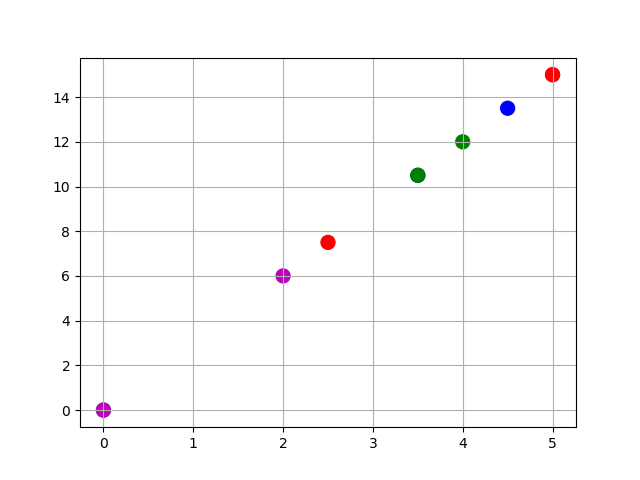
\includegraphics{3x.png}
\end{figure}
Οπότε τα σημεία ανήκουν σε ημιευθεία η οποία περνάει από την αρχή των αξόνων.